\documentclass[a4paper, 10pt, twoside]{article}
\usepackage[left=2cm, right=2cm, top=2cm, bottom=3cm]{geometry}
\usepackage{amsmath}
\usepackage{bm}
\usepackage[shortlabels]{enumitem}
\usepackage{bbold}
\usepackage{cases}
\usepackage{systeme}
\usepackage{graphicx}
\usepackage{booktabs}

\begin{document}

\title{Machine Learning - Theoretical exercise 4}
\author{T\'eo Bouvard}
\maketitle

\section*{Problem 1}
\begin{enumerate}[a)]
    \item We have the same number of training samples for classes $\omega_1$ and $\omega_2$, thus the prior probabilities are equal for both classes i.e. $P(\omega_1)=0.5$ and $P(\omega_2)=0.5$

          \begin{center}
              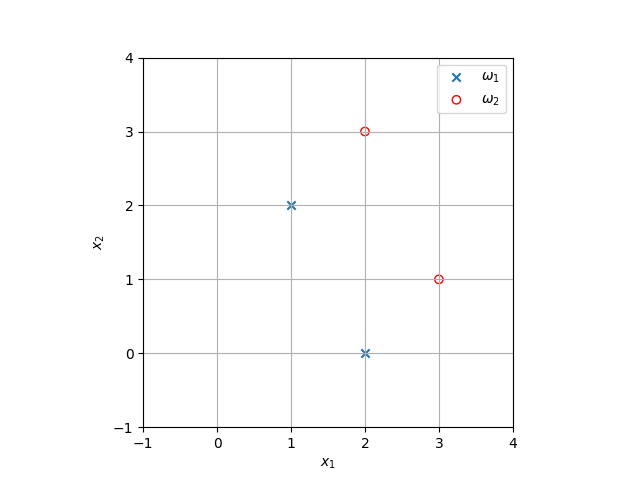
\includegraphics[width=0.5\textwidth]{img/graph1.png}
          \end{center}

    \item We compute $\theta$ according to the LS-method.
          \begin{align}
              \theta = (X^TX)^{-1}X^Ty
          \end{align}
          where
          \begin{align*}
              X =
              \begin{bmatrix}
                  1 & 2 & 1 \\
                  2 & 0 & 1 \\
                  3 & 1 & 1 \\
                  2 & 3 & 1 \\
              \end{bmatrix}^T
               &  &
              y =
              \begin{bmatrix}
                  1 \\ 1 \\ -1 \\ -1
              \end{bmatrix}
          \end{align*}
          The steps to solve this equation are shown below.
          \begin{align*}
              X^TX           & =
              \begin{bmatrix}
                  18 & 11 & 8 \\
                  11 & 14 & 6 \\
                  8  & 6  & 4 \\
              \end{bmatrix} \\
              (X^TX)^{-1}    & =
              \begin{bmatrix}
                  -\frac{5}{9}   & \frac{1}{9}  & -\frac{23}{18} \\
                  \frac{1}{9}    & \frac{2}{9}  & -\frac{5}{9}   \\
                  -\frac{23}{18} & -\frac{5}{9} & \frac{131}{36} \\
              \end{bmatrix} \\
              (X^TX)^{-1}X^T & =
              \begin{bmatrix}
                  -\frac{1}{2} & -\frac{1}{6}   & \frac{1}{2}  & \frac{1}{6}   \\
                  0            & -\frac{1}{3}   & 0            & \frac{1}{3}   \\
                  \frac{5}{4}  & -\frac{13}{12} & -\frac{3}{4} & -\frac{7}{12} \\
              \end{bmatrix} \\
              \bm{\theta}    & =
              \begin{bmatrix}
                  -\frac{4}{3} \\
                  -\frac{2}{3} \\
                  \frac{11}{3} \\
              \end{bmatrix} \\
          \end{align*}
          To determine the decision boundary, we find the root of the discriminant function.
          \begin{align*}
              g(x) = 0                                              \\
              -\frac{4}{3} x_1 - \frac{2}{3} x_2 + \frac{11}{3} = 0 \\
              x_2 = -2x_1 + \frac{11}{2}
          \end{align*}
          \begin{center}
              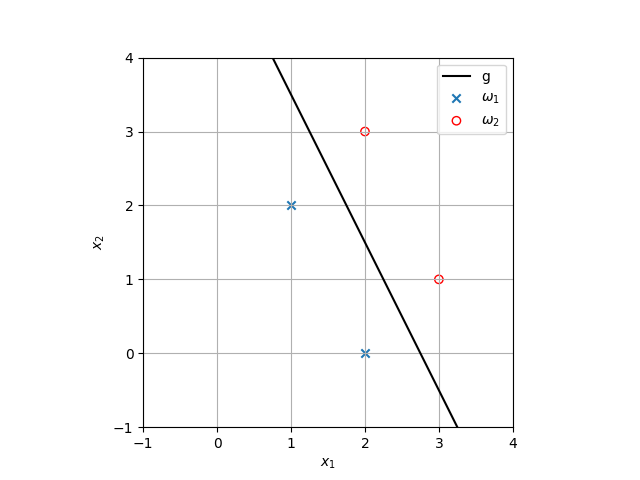
\includegraphics[width=0.5\textwidth]{img/graph2.png}
          \end{center}

    \item If we set $y_4=-0.5$, we reduce the weight of the fourth training sample, which modifies $\theta$.
          \begin{align*}
              \theta' =
              \begin{bmatrix}
                  -\frac{5}{4} \\
                  -\frac{1}{2} \\
                  \frac{27}{8} \\
              \end{bmatrix}
          \end{align*}
          Because $\theta' \neq \theta$, the decision boundary also changes.
          \begin{align*}
              g'(x) = 0                                             \\
              -\frac{5}{4} x_1 - \frac{1}{2} x_2 + \frac{27}{8} = 0 \\
              x_2 = -\frac{5}{2} x_1 + \frac{27}{4}
          \end{align*}
          \begin{center}
              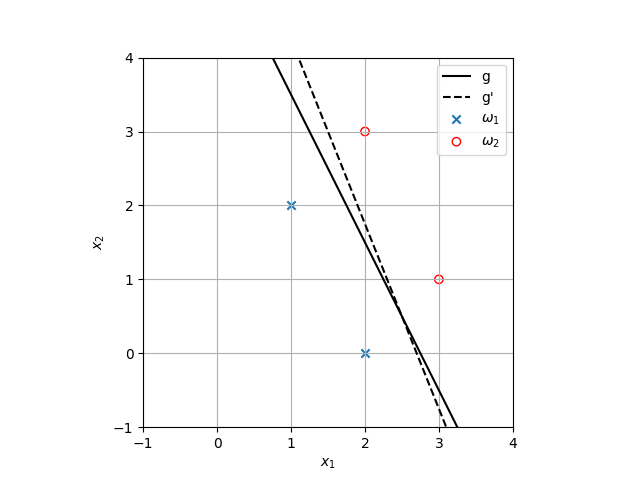
\includegraphics[width=0.5\textwidth]{img/graph3.png}
          \end{center}
          We can see that decreasing the weight of a training sample moves the decison boundary closer to it.

    \item We now compute $\theta$ with the LMS-method. We use $\mu$ to denote the the learning rate. The descent vector at each iteration is denoted $\nabla$.

          Initialization

          \begin{align*}
              \mu^{(0)} = 0.5
               &  &
              \bm{\theta}^{(0)} =
              \begin{bmatrix}
                  1 \\ 1 \\ 1
              \end{bmatrix}
               &  &
              \theta = 1
          \end{align*}

          Iteration 1

          \begin{align*}
              \nabla
               & =
              \mu^{(1)}(y_1-\bm{\theta}^{(0)T}y_1x_1)y_1x_1 \\
               & =
              \frac{0.5}{1}
              \left(
              \begin{bmatrix}
                      1
                  \end{bmatrix}
              -
              \begin{bmatrix}
                      1 & 1 & 1
                  \end{bmatrix}
              \begin{bmatrix}
                      1
                  \end{bmatrix}
              \begin{bmatrix}
                      1 \\ 2 \\ 1
                  \end{bmatrix}
              \right)
              \begin{bmatrix}
                  1
              \end{bmatrix}
              \begin{bmatrix}
                  1 \\ 2 \\ 1
              \end{bmatrix}                    \\
               & =
              -\frac{3}{2}
              \begin{bmatrix}
                  1 \\ 2 \\ 1
              \end{bmatrix}
          \end{align*}

          \begin{align*}
              \begin{vmatrix}
                  \nabla
              \end{vmatrix} = \frac{3\sqrt{6}}{2} \approx 3.7 > \theta
          \end{align*}

          $\begin{vmatrix} \nabla \end{vmatrix}$ is greater than the threshold, so $ \bm{\theta} $ is updated, and we will need to loop through all samples again for the next epoch.

          \begin{align*}
              \bm{\theta}^{(1)}
               & = \bm{\theta}^{(0)} + \nabla \\
               & = -\frac{1}{2}
              \begin{bmatrix}
                  1 \\ 4 \\ 1
              \end{bmatrix}
          \end{align*}

          Iteration 2

          \begin{align*}
              \nabla
               & =
              \mu^{(2)}(y_2-\bm{\theta}^{(1)T}y_2x_2)y_2x_2 \\
               & =
              \frac{0.5}{2}
              \left(
              \begin{bmatrix}
                      1
                  \end{bmatrix}
              -
              \begin{bmatrix}
                      -\frac{1}{2} & -2 & -\frac{1}{2}
                  \end{bmatrix}
              \begin{bmatrix}
                      1
                  \end{bmatrix}
              \begin{bmatrix}
                      2 \\ 0 \\ 1
                  \end{bmatrix}
              \right)
              \begin{bmatrix}
                  1
              \end{bmatrix}
              \begin{bmatrix}
                  2 \\ 0 \\ 1
              \end{bmatrix}                    \\
               & =
              \begin{bmatrix}
                  \frac{5}{4} \\ 0 \\ \frac{5}{8}
              \end{bmatrix}
          \end{align*}

          \begin{align*}
              \begin{vmatrix}
                  \nabla
              \end{vmatrix} = \frac{5\sqrt{5}}{8} \approx 1.4 > \theta
          \end{align*}

          $\begin{vmatrix} \nabla \end{vmatrix}$ is greater than the threshold, so $ \bm{\theta} $ is updated.

          \begin{align*}
              \bm{\theta}^{(2)}
               & = \bm{\theta}^{(1)} + \nabla \\
               & =
              \begin{bmatrix}
                  \frac{3}{4} \\ -2 \\ \frac{1}{8}
              \end{bmatrix}
          \end{align*}

          Iteration 3

          \begin{align*}
              \nabla
               & =
              \mu^{(3)}(y_3-\bm{\theta}^{(2)T}y_3x_3)y_3x_3 \\
               & =
              \frac{0.5}{3}
              \left(
              \begin{bmatrix}
                      -1
                  \end{bmatrix}
              -
              \begin{bmatrix}
                      \frac{3}{4} & -2 & \frac{1}{8}
                  \end{bmatrix}
              \begin{bmatrix}
                      -1
                  \end{bmatrix}
              \begin{bmatrix}
                      3 \\ 1 \\ 1
                  \end{bmatrix}
              \right)
              \begin{bmatrix}
                  -1
              \end{bmatrix}
              \begin{bmatrix}
                  3 \\ 1 \\ 1
              \end{bmatrix}                    \\
               & =
              \begin{bmatrix}
                  \frac{5}{16} \\ \frac{5}{48} \\ \frac{5}{48}
              \end{bmatrix}
          \end{align*}

          \begin{align*}
              \begin{vmatrix}
                  \nabla
              \end{vmatrix} = \frac{5\sqrt{11}}{48} \approx 0.3 < \theta
          \end{align*}

          $\begin{vmatrix} \nabla \end{vmatrix}$ is smaller than the threshold, so $ \bm{\theta} $ is not updated and we continue with the third sample. The rest of the computations were done programmaticaly.
          After the $12^{th}$ iteration, the algorithm converges and exits with the following result.

          \begin{align*}
              \bm{\theta} \approx
              \begin{bmatrix}
                  0.79 \\ -0.42 \\ 0.36
              \end{bmatrix}
          \end{align*}

          If we plot the resulting decision boundary, we observe that the converged value of $\bm{\theta}$ does not discriminate between the classes.

          \begin{center}
              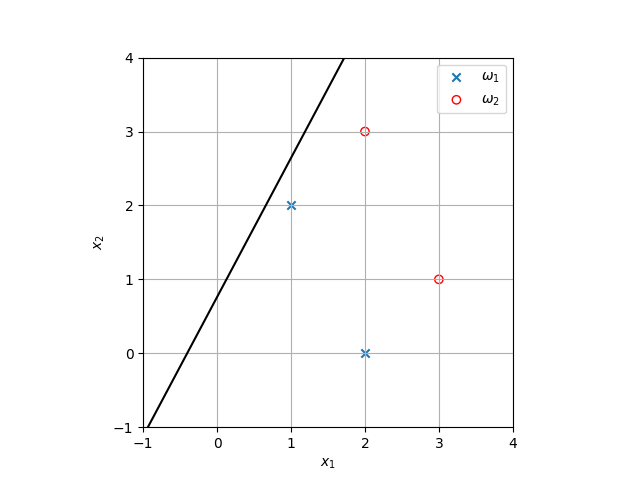
\includegraphics[width=0.5\textwidth]{img/graph4.png}
          \end{center}

\end{enumerate}

\section*{Problem 2}

\begin{enumerate}[a)]
    \item An analytical solution to the equation $\bm{X\theta}= \bm{y}$ would be to find the inverse of $\bm{X}$ and compute $\bm{\theta} = \bm{X^{-1}y}$ directly. However, this solution assume that $\bm{X}$ is invertible. In practice $\bm{X}$ is often rectangular, with more rows (samples) than columns (features). Trying to find an exact solution would lead to have more equations than unknowns which is not solvable in general.

    \item  In order to find $\bm{\theta}$ minimizing the function $\Vert \bm{X \theta - y} \Vert^2$, we can differentiate this function with respect to $\bm{\theta}$ and find its root.

          \begin{align*}
              \frac{\partial \Vert \bm{X \theta} - \bm{y} \Vert^2}{\partial \bm{\theta}}
              = 2 \bm{X}^T(\bm{X \theta - y})
          \end{align*}

          We now set the derivative to zero.

          \begin{align*}
              2 \bm{X}^T(\bm{X \theta} - \bm{y}) & = 0                                   \\
              \bm{X}^T\bm{X \theta }             & = \bm{X^T y}                          \\
              \bm{\theta}                        & = ( \bm{X}^T \bm{X} )^{-1} \bm{X^T y} \\
          \end{align*}

          In this case, $\bm{X}^T \bm{X}$ is guaranteed to be invertible because it is a square symmetric matrix.

    \item Let $\bm{\theta_*}$ be the value of $\bm{\theta}$ minimizing the squared error. We can rewrite the distance function as such.

          \begin{align*}
              \Vert \bm{X \theta_* - y} \Vert^2 = \Vert \bm{X} (\bm{X}^T\bm{X})^{-1}\bm{X}^T \bm{y} - \bm{y} \Vert^2
          \end{align*}

    \item For the problem to be lineraly separable, the distance function should be equal to zero.

          \begin{align*}
              \Vert \bm{X} (\bm{X}^T\bm{X})^{-1}\bm{X}^T \bm{y} - \bm{y} \Vert^2 = 0
              \implies
              \bm{X} (\bm{X}^T\bm{X})^{-1}\bm{X}^T \bm{y} = \bm{y}
              \implies
              \bm{X} (\bm{X}^T\bm{X})^{-1}\bm{X}^T = \bm{I}
          \end{align*}

\end{enumerate}

\section*{Problem 3}

\begin{enumerate}[a)]
    \item Samples are labeled as +1 if they belong to $\omega_1$ and -1 if they belong to $\omega_2$.

          \begin{align*}
              y_1 = +1 &  & y_2 = +1 &  & y_3 = -1
          \end{align*}

    \item For each sample, we draw the decision boundary $y_i \bm{\theta}_T x_i = 0$. This "normalization" of each sample by its class label simplifies the analysis as we only have to check that $y_i \bm{\theta}_T x_i > 0$ to conclude that the classification is correct.

          \begin{figure}[h]
              \centering
              \begin{minipage}[t]{0.32\textwidth}
                  \centering
                  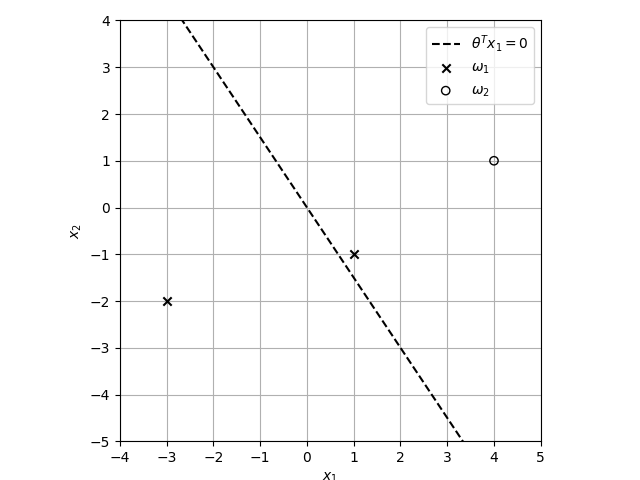
\includegraphics[width=\textwidth]{img/graph5.png}
              \end{minipage}\hfill
              \begin{minipage}[t]{0.32\textwidth}
                  \centering
                  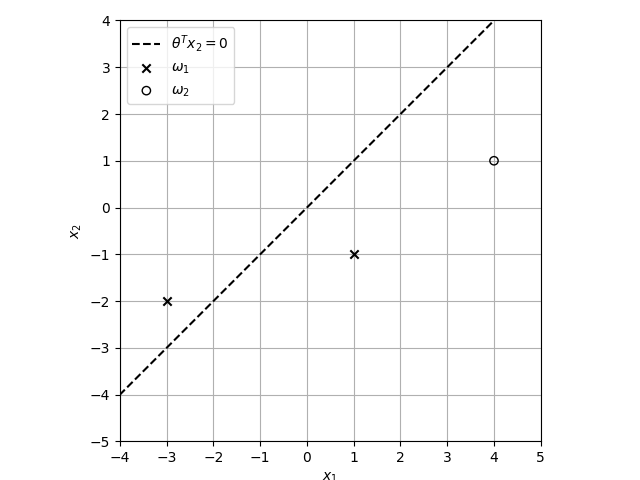
\includegraphics[width=\textwidth]{img/graph7.png}
              \end{minipage}\hfill
              \begin{minipage}[t]{0.32\textwidth}
                  \centering
                  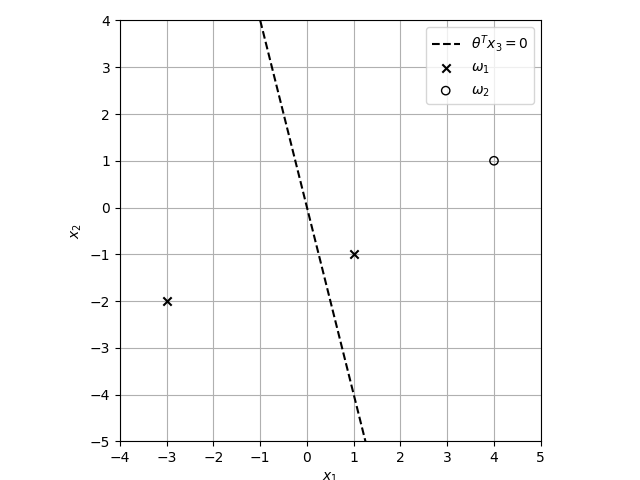
\includegraphics[width=\textwidth]{img/graph9.png}
              \end{minipage}
          \end{figure}

    \item The normalization we used also simplifies the visualization as we only need to consider the intersection of all positive regions to find the solution region.If we colour the positive side of the discriminant function in red and the negative side in blue, we get the following regions.

          \begin{figure}[h]
              \centering
              \begin{minipage}[t]{0.32\textwidth}
                  \centering
                  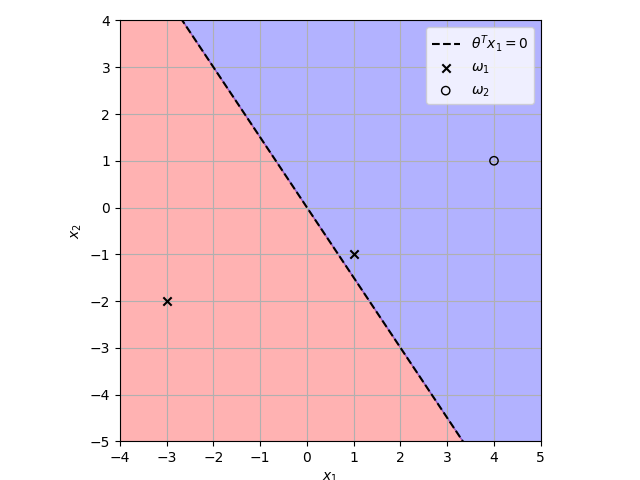
\includegraphics[width=\textwidth]{img/graph6.png}
              \end{minipage}\hfill
              \begin{minipage}[t]{0.32\textwidth}
                  \centering
                  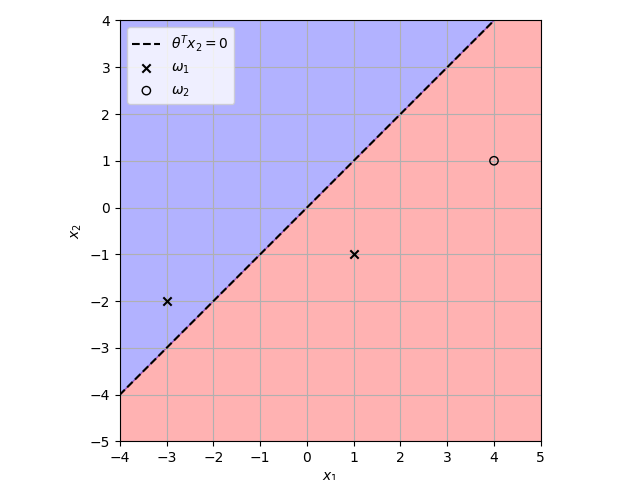
\includegraphics[width=\textwidth]{img/graph8.png}
              \end{minipage}\hfill
              \begin{minipage}[t]{0.32\textwidth}
                  \centering
                  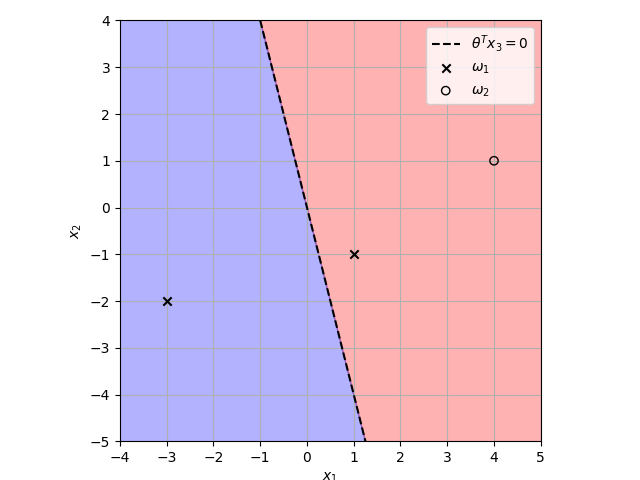
\includegraphics[width=\textwidth]{img/graph10.png}
              \end{minipage}
          \end{figure}

          If we superpose the three previous plots, we can identify the solution region by color addition. The solution region is the one having the most vivid red color.

          \begin{center}
              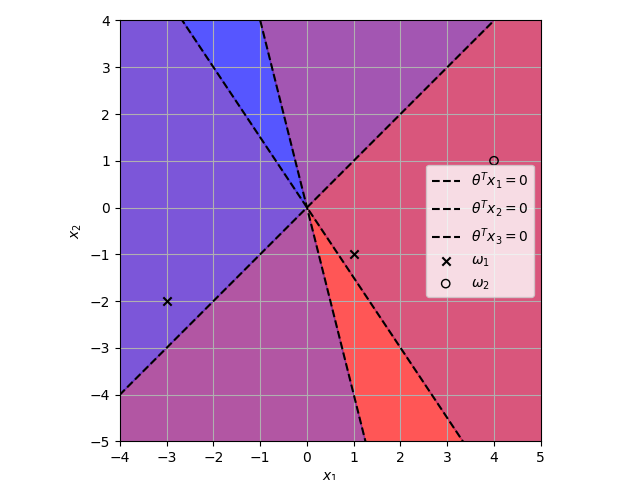
\includegraphics[width=0.7 \textwidth]{img/solution_region.png}
          \end{center}

    \item We apply the Batch Perceptron algorithm with a constant learning rate. Let $X_i$ be the set of misclassified samples at iteration $i$. We identify the misclassified samples by checking if $y_i \bm{\theta}^{(i)^T} > \theta$

          Initialization

          \begin{align*}
              \bm{\theta}^{(1)} = \begin{bmatrix} 0 & 0\end{bmatrix}^T &  & \mu = 1 &  & \theta = 0
          \end{align*}

          Iteration 1

          \begin{align*}
              \bm{\theta}^{(1)^T} x_1 = 0 &  & \bm{\theta}^{(1)^T} x_2 = 0 &  & \bm{\theta}^{(1)^T} x_3 = 0 &  & \implies &  & X = \{x_1, x_2, x_3 \} \\
          \end{align*}

          $X$ is not empty, so we should update $\bm{\theta}$

          \begin{align*}
              \bm{\theta}^{(2)} & = \bm{\theta}^{(1)} + \mu (y_1 x_1 + y_2 x_2 + y_3 x_3)                                                             \\
                                & = \begin{bmatrix} 0 \\ 0 \end{bmatrix} + \begin{bmatrix} -3 \\ -2 \end{bmatrix} + \begin{bmatrix} 1 \\ -1 \end{bmatrix} - \begin{bmatrix} -4 \\ -1 \end{bmatrix} \\
                                & = \begin{bmatrix} 2 \\ -2 \end{bmatrix}
          \end{align*}

          Iteration 2
          \begin{align*}
              \bm{\theta}^{(2)^T} x_1 = -2 &  & \bm{\theta}^{(2)^T} x_2 = 4 &  & \bm{\theta}^{(2)^T} x_3 = 6 &  & \implies &  & X = \{ x_1 \} \\
          \end{align*}

          $X$ is not empty, so we should update $\bm{\theta}$

          \begin{align*}
              \bm{\theta}^{(3)} & = \bm{\theta}^{(2)} + \mu (y_1 x_1)                       \\
                                & = \begin{bmatrix} 2 \\ -2 \end{bmatrix} + \begin{bmatrix} -3 \\ -2 \end{bmatrix} \\
                                & = \begin{bmatrix} -1 \\ -4 \end{bmatrix}
          \end{align*}

          Iteration 3
          \begin{align*}
              \bm{\theta}^{(3)^T} x_1 = 11 &  & \bm{\theta}^{(3)^T} x_2 = 3 &  & \bm{\theta}^{(3)^T} x_3 = -8 &  & \implies &  & X = \{ x_3 \} \\
          \end{align*}

          $X$ is not empty, so we should update $\bm{\theta}$

          \begin{align*}
              \bm{\theta}^{(4)} & = \bm{\theta}^{(3)} + \mu (y_3 x_3)                       \\
                                & = \begin{bmatrix} -1 \\ -4 \end{bmatrix} - \begin{bmatrix} -4 \\ -1 \end{bmatrix} \\
                                & = \begin{bmatrix} 3 \\ -3 \end{bmatrix}
          \end{align*}

          At iteration 8, we end up with $\bm{\theta}^{(8)} = \begin{bmatrix} 2 & -7 \end{bmatrix}^T $.

          \begin{align*}
              \bm{\theta}^{(8)^T} x_1 = 8 &  & \bm{\theta}^{(3)^T} x_2 = 9 &  & \bm{\theta}^{(3)^T} x_3 = 1 &  & \implies &  & X = \emptyset \\
          \end{align*}

          We can see that all samples are correctly classified with this value of $\bm{\theta}$.

    \item We now apply the Batch Perceptron algorithm, but we decrease decrease the learning rate at each iteration. We get the following results.

          \begin{table}[h]
              \centering
              \begin{tabular}{cccc}
                  i & $\bm{\theta}^T$              & $X$                   & $\vert \mu \sum_{x \in X} y_i x_i \vert$ \\
                  \toprule
                  1 & $\begin{bmatrix} 0 & 0 \end{bmatrix}$ & $\{ x_1, x_2, x_3 \}$ & 2.82                                     \\
                  2 & $\begin{bmatrix} 2 & -2 \end{bmatrix}$ & $\{ x_1 \}$           & 1.80                                     \\
                  3 & $\begin{bmatrix} 0.5 & -3 \end{bmatrix}$ & $\{ x_3 \}$           & 1.37                                     \\
                  4 & $\begin{bmatrix} 1.8 & -2.7 \end{bmatrix}$ & $\{ x_1 \}$           & 0.90                                     \\
                  5 & $\begin{bmatrix} 1.1 & -3.2 \end{bmatrix}$ & $ \emptyset $         & 0                                        \\
              \end{tabular}
          \end{table}

          We can see that decreasing the learning rate at each step reduces the steps needed to converge to the solution region.


\end{enumerate}

\end{document}
